\sectioncentered*{Введение}
\addcontentsline{toc}{section}{Введение}
\label{sec:intro}
При цифровой обработке изображений непрерывный динамический диапазон значений яркости делится на ряд дискретных уровней. Эта процедура называется \textit{квантованием}. Её суть заключается в преобразовании непрерывной переменной $x$  в дискретную переменную $x_{\x{кв}}$, принимающую конечное множество значений $\left\lbrace  r_{1}, \dots , r_{L}  \right\rbrace$. Эти значения называются уровнями квантования. В общем случае преобразование выражается ступенчатой функцией на рисунке \ref{fig:quan_signal}. Если интенсивность  отсчета изображения принадлежит интервалу $\left( d_{j} d_{j+1} \right] $  (т.е., когда $d_{j} < x \le d_{j} $), то исходный отсчет заменяется на уровень квантования $r_{j}$ , где $d_{j}, j=\overline{ 1, L+1 } $ "---  пороги квантования. При этом полагается, что динамический диапазон значений яркости ограничен и равен $\left[ d_{1}, d_{L+1}\right]$.
\begin{figure}[h]
    \centering
        \begin{tikzpicture}
        \centering
        \begin{axis}[
        axis x line=center,
        axis y line=center,
        yticklabels={,,},
        xticklabels={,,},
        xtick={ -3,-2,...,3},
        ytick={ -3,-2,...,3},
        xlabel={$d$},
        ylabel={$r$},
        xmin=-4,
        xmax=4,
        ymin=-4,
        ymax=4]
        \addplot [blue] table {
            x f(x)
            -3 -2.5
            -2 -2.5
            -2 -1.5
            -1 -1.5
            -1 -0.5
            -0 -0.5
            -0 0.5
            1 0.5
            1 1.5
            2 1.5
            2 2.5
            3 2.5
            
            
        };
        \end{axis}
        \end{tikzpicture}
 \caption{Функция, описывающая квантование}
\label{fig:quan_signal}
\end{figure}
%вставить рисунок
%Рис. 1.  Функция, описывающая квантование
Задача построения квантователя состоит в определении значений порогов $d_{j}$  и уровней $r_{j}$. Простейший способ решения этой задачи состоит в разбиении динамического диапазона на одинаковые интервалы. Однако такое решение не является наилучшим.
 \cite[c.~20]{Gruzman_2002}

Обычно квантование применяется для преобразования непрерывной величины в дискретную, например в следующих операциях:
\begin{itemize}
    \item оцифровка изображения;
    \item растеризация векторной графики.
\end{itemize}
В представленной курсовой работе происходит преобразование дискретной величины в дискретную, но с уменьшением количества уровней квантования.

Однако важен не только вышеописанный процесс, а также последующие за ним кодирование полученных данных. В этой работе был применен алгоритм \textit{кодирования длин серий} (англ. run-length encoding, RLE). Идея такого подхода к сжатию данных заключается в следующем: если элемент данных $d$ повторяется $n$ раз подряд в входной последовательности, то заменить $n$ вхождений одной парой $nd$. $n$ последовательных вхождений элемента данных $d$ называется серией длинны $n$. \cite[c.~22]{Salomon_2007}

Вышеописанные преобразования изображения позволяет сократить объем обрабатываемых данных при дальнейшем анализе, что в свою очередь увеличивает скорость обработки. Также в некоторых случаях в полученных данных возможно найти закономерности упрощающие последующие операции над изображением.
 
Рассматриваемый квантователь реализован  для изображений получаемых с определенной камеры. Как видно на рисунке \ref{fig:videofur1} получаемые изображения весьма специфичны. В ходе работы был разработан алгоритм учитывающий особенности входных данных. 
\begin{figure}[h]
    \centering
    \begin{subfigure}{\textwidth}
        \centering
        
\includegraphics[width = \textwidth]{videofur_25.jpg}
        \caption{}
    \end{subfigure}    
    \begin{subfigure}{\textwidth}
        \centering
        
\includegraphics[width = \textwidth]{videofur_26.jpg}
        \caption{}
    \end{subfigure} 
\begin{subfigure}{\textwidth}
    \centering
    
\includegraphics[width = \textwidth]{videofur_27.jpg}
    \caption{}
\end{subfigure} 
\begin{subfigure}{\textwidth}
    \centering
    
\includegraphics[width = \textwidth]{videofur_28.jpg}
    \caption{}
\end{subfigure} 
    \caption{Примеры кадров}
    \label{fig:videofur1}
\end{figure}

\section{Описание среды разработки}
\label{sec:env_description}
В данном разделе будут рассмотрены различные инструменты используемые в ходе выполнения работы, их процесс установки и специфика использования. Также будет произведен краткий сравнительный анализ аналогичных средств, будет дано обоснование выбора именно тех средств, которые использованы в данной работе. 
\subsection{Visual Studio}
\label{sub:env_description:vs}
\textit{Microsoft Visual Studio} — линейка продуктов компании Microsoft, включающих интегрированную среду разработки программного обеспечения и ряд других инструментальных средств. Данные продукты позволяют разрабатывать как консольные приложения, так и приложения с графическим интерфейсом, в том числе с поддержкой технологии Windows Forms, а также веб-сайты, веб-приложения, веб-службы как в родном, так и в управляемом кодах для всех платформ, поддерживаемых Windows, Windows Mobile, Windows CE, .NET Framework, Xbox, Windows Phone .NET Compact Framework и Silverlight.

Visual Studio является одним из лидеров среди интегрированных сред разработки на языке C++. Высокая популярность данной среды выражается в огромном мировом сообществе разработчиков использующих её. Благодаря этому сообществу у разработчика, применяющего Visual Studio для решения своих задач, появляется возможность более быстрого решения часто возникающих проблем. Также большинство сторонних библиотек и других инструментов имеют версию специально выпущенную для Visual Studio.

Visual Studio является коммерческим проектом, однако для некоммерческой разработки предоставляется специализированная версия Community. По сравнению с версией Professional данная версия обладает ограниченным функционалом, однако в работе этот функционал не использовался. Поэтому разработка велась на версии Visual Studio 2017 Community RC. Для начала установки требуется скачать установщик с официального сайта Microsoft \cite{vs_downolad}. Там располагается ссылка для скачивания, как на рисунке \ref{fig:vs_downolad}. 
\begin{figure}[h]
    \centering
     \begin{subfigure}{0.45\textwidth}  
         \centering     
        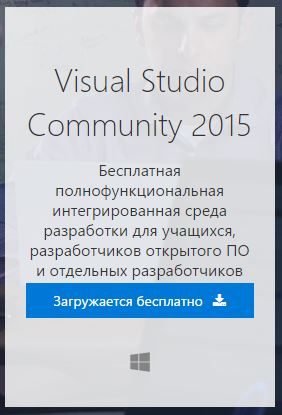
\includegraphics[width = \textwidth]{vs_download.JPG}
        \caption{}
        \label{fig:vs_downolad}
    \end{subfigure}
    \begin{subfigure}{0.45\textwidth}  
        \centering
        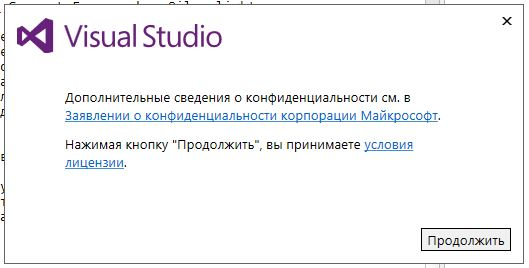
\includegraphics[width = \textwidth]{vs_licence.JPG}
        \caption{}
        \label{fig:vs_licence}
    \end{subfigure}
    \caption{а "--- Ссылка для загрузки установщика; б "--- окно принятия лицензионного соглашения}
    \label{fig:vs_install1}
\end{figure}
Запускаем скачанный файл, он запустит процесс установки. Предварительно попросив принять условия лицензионного соглашения. Для перехода на следующий этап требуется нажать кнопку \textit{"Продолжить"} как показано на рисунке \ref{fig:vs_licence}. После этого запустится Visual Studio Installer, который служит для установки и модернизации различных версий Visual Studio 2017.
\begin{figure}[h]
    \centering   
    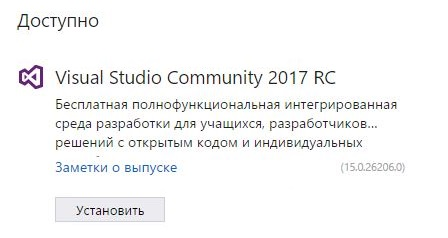
\includegraphics[width = 0.5\textwidth]{vs_install.JPG} 
    \caption{Выбор требуемой версии Visual Studio}
    \label{fig:vs_install2}
\end{figure}
После выбора нужной версии Visual Studio и нажатия кнопки \textit{"Установить"} откроется окно выбора комплектации среды разработки и дополнительных приложений, показное на рисунке \ref{fig:vs_install_chouse}. Для работы с данным проектом достаточно выбрать пункт \textit{"Разработка классических приложений на C++"} и Предпочтительные языковые пакеты на вкладке \textit{"Языковые пакеты"}. Однако в зависимости от потребностей пользователя можно установить и дополнительные пакеты.
\begin{figure}[h]
    \centering   
    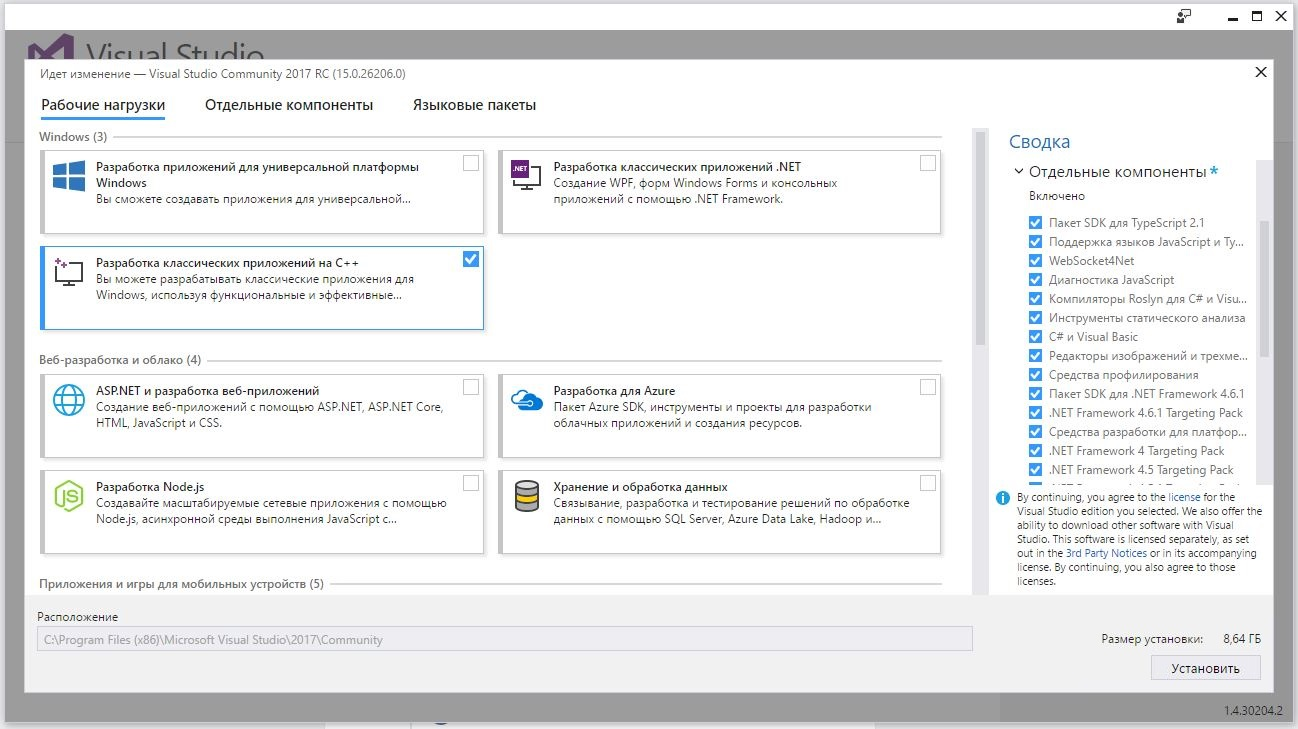
\includegraphics[width = \textwidth]{vs_install_chouse.JPG} 
    \caption{Окно выбора комплектации среды разработки и дополнительных приложений }
    \label{fig:vs_install_chouse}
\end{figure} 
\begin{figure}[h]
    \centering   
    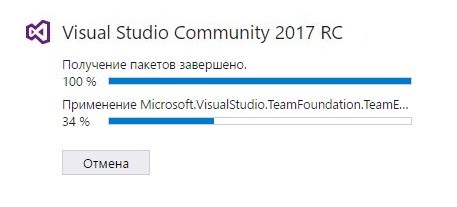
\includegraphics{vs_install2.JPG} 
    \caption{Процесс скачивания и установки Visual Studio}
    \label{fig:vs_install_progress}
\end{figure} 
Нажатие на кнопку \textit{"Установить"} запустит процесс установки Visual Studio. После его завершения можно запустить среду разработки. При первом запуске запрашивается вход под аккаунтом Microsoft, если он еще не зарегистрирован то можно или пропустить данный шаг и работать в неавторизированной версии или зарегистрироваться на официальном сайте Microsoft.

\subsection{OpenCV}
\label{sub:env_description:opencv}
\textit{OpenCV} "--- выпущенная под лицензией BSD библиотека, а следовательно бесплатная для коммерческого и академического использования. Она имеет интерфейсы для C++, C, Python и Java. Поддерживает такие операционные системы как: Windows, Linux, Mac OS, Android и IOS. OpenCV была разработана для обеспечения эффективных вычислений с ориентацией на приложения реального времени. Написанная на оптимизированном C/C++, библиотека способна использовать преимущества многоядерной обработки. Работая вместе с OpenCL она может использовать возможности аппаратного ускорения. Используемая во всем мире, OpenCV насчитывает более 47 тысячи человек в сообществе пользователей и более девяти миллионов скачиваний. Применяется в различных сферах, начиная с интерактивного искусства, обнаружения мин или построения спутниковых карт до современной робототехники. \cite{opencv_offical}

\textit{OpenCV} "--- наиболее полная, постоянно развивающаяся библиотека для обработки изображений. Огромное количество функций реализующих различные алгоритмы для обработки и анализа изображений позволяют сосредоточится на решении конкретной задачи, не отвлекаясь на написание заново уже известных классических алгоритмов. Единственным конкурентом OpenCV в сфере цифровой обработки изображений является MATLAB. Однако он больше подходит для прототипной разработки и исследований алгоритмов из-за удобства отладки, в скорости работы конечного приложения MATLAB сильно уступает возможностям OpenCV. Исходя из этих преимуществ OpenCV выбрана в качестве основного инструмента для разработки данного проекта. 

